\section{ロボットモデル}
\label{sec:robot_model}

本研究で使用する二足歩行ロボットは，CHIDORI と呼ばれる人型ロボットである（\cref{fig:chidori}）．CHIDORI は，全身の重心運動および支持脚の力学的挙動を精密に制御可能な構造を有しており，歩行制御アルゴリズムの検証を目的としたシミュレーションおよび実機実験に用いられている．本研究では，この CHIDORI をシミュレーション上で再現し実験を行った．シミュレーションに用いた CHIDORI の主要な物理パラメータを \cref{tab:robot_spec} に示す．

\begin{figure}[htbp]
  \centering
  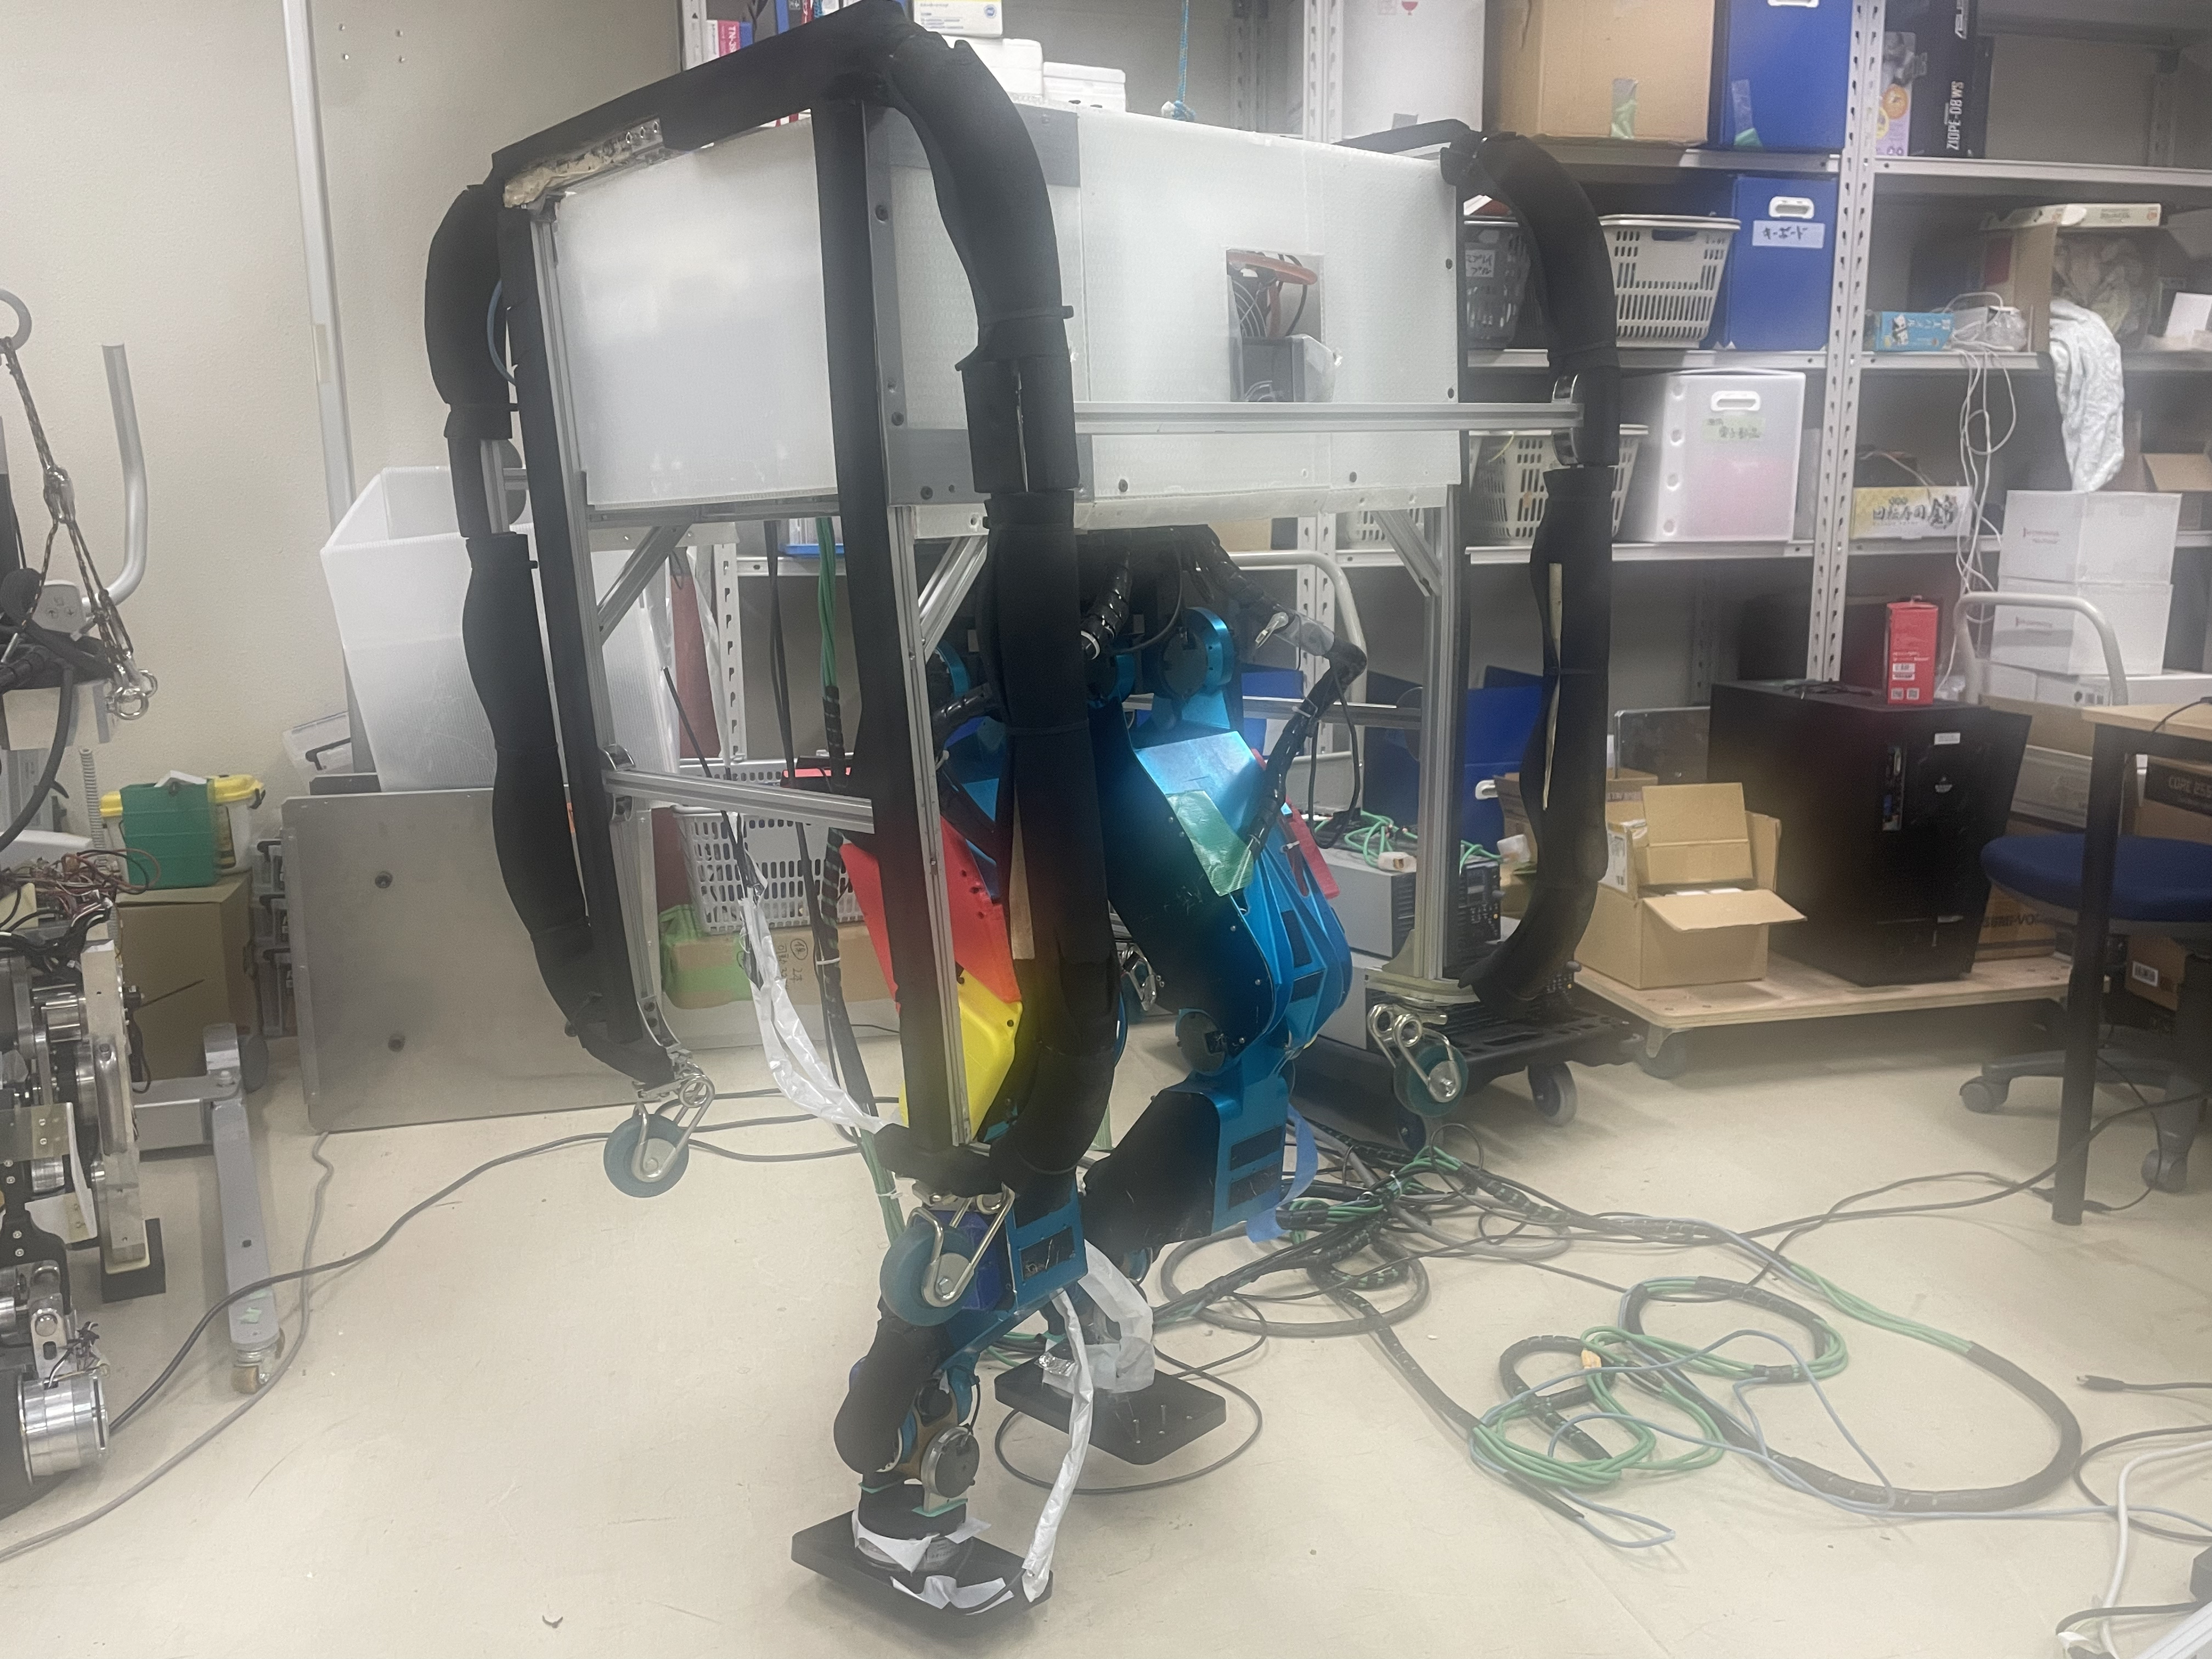
\includegraphics[width=0.5\linewidth]{images/chidori.png}
  \caption{CHIDORI ロボット}
  \label{fig:chidori}
\end{figure}

\begin{figure}[htbp]
  \centering
  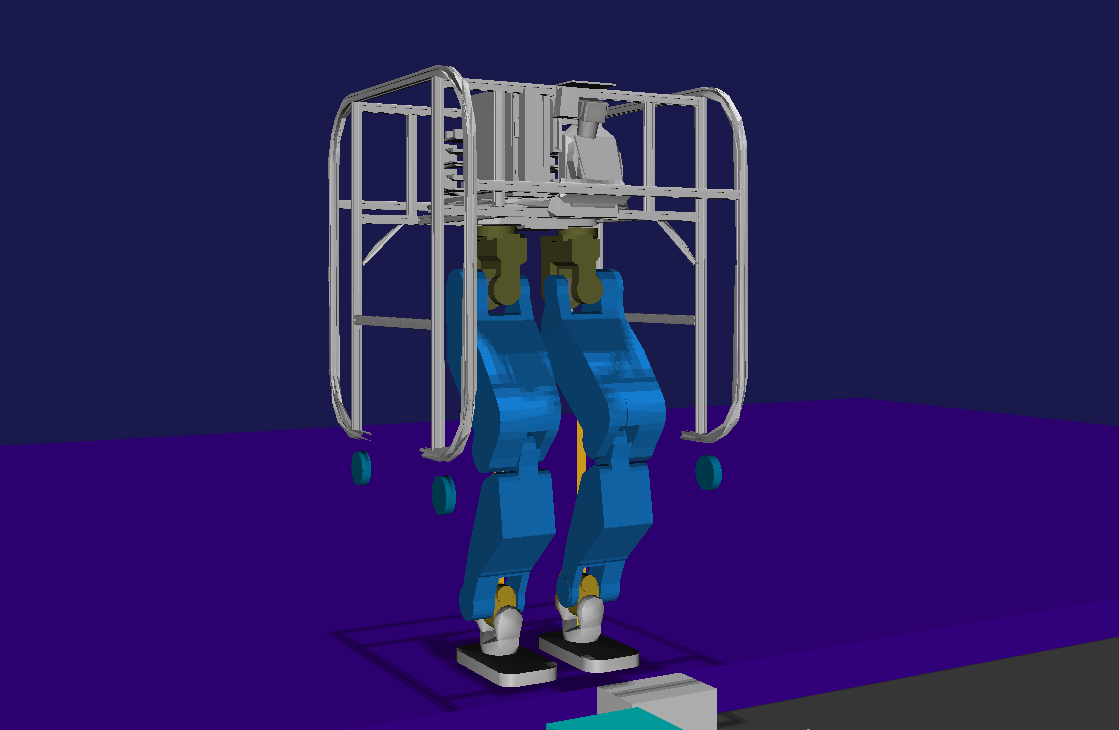
\includegraphics[width=0.5\linewidth]{images/sim_chidori.png}
  \caption{シミュレーション上で再現したCHIDORI ロボットモデル}
  \label{fig:sim_chidori}
\end{figure}

\begin{table}[t]
  \centering
  \caption{CHIDORI ロボットモデルの主要諸元}
  \label{tab:robot_spec}
  \begin{tabular}{l c}
    \hline
    項目 & 値 \\
    \hline
    全質量 & $67.04$\,kg \\
    自由度数（全身） & $23$ \\
    自由度数（下半身） & $12$ \\
    片脚自由度数 & $6$ \\
    足裏サイズ（長さ $\times$ 幅） & $260 \times 134$\,mm \\
    標準姿勢時 CoM 高さ & $0.7039$\,m \\
    \hline
  \end{tabular}
\end{table}
